\documentclass[conference]{IEEEtran}
\usepackage{amsmath,amssymb,booktabs,graphicx,xcolor}
\usepackage[hidelinks]{hyperref}
\usepackage{url}
\usepackage{balance}
\usepackage{iftex}
\ifXeTeX
\usepackage{fontspec}
\setmainfont{texgyretermes-regular.otf}[BoldFont=texgyretermes-bold.otf,ItalicFont=texgyretermes-italic.otf,BoldItalicFont=texgyretermes-bolditalic.otf]
\setsansfont{texgyreheros-regular.otf}[BoldFont=texgyreheros-bold.otf,ItalicFont=texgyreheros-italic.otf]
\setmonofont{texgyrecursor-regular.otf}[BoldFont=texgyrecursor-bold.otf]
\fi
\definecolor{forest}{RGB}{32,75,64}
\title{Maintaining Source-Linked Evidence Views for Agent Memory}
\author{}
\begin{document}
\maketitle
\begin{abstract}
An agent's context combines records that cost different numbers of tokens and may outlive the repository state they describe. We demonstrate two source-linked SQLite views. One assembles tool evidence under a token budget and explains when an exclusion changes the optimal packet. The other tracks previously read code through editor-confirmed changes and checks displayed coordinates against file contents. On ISETrace a learned selector attained 83.07\% full evidence support against 81.19\% for first-fit on the same native ranking. On 1,071 code edits from 13 held-out issues, range-level invalidation preserved 302 complete packets against two under file-level invalidation. All 25,912 retained lines checked on the edited paths matched their subsequent file snapshots. Halfway through the event history, our first-fit graph reader recovered 84.73\% complete support against 81.38\% for the stronger native graph reader. Visitors can exclude a dependency, relocate a surviving block and inspect incorrect source coordinates.

\end{abstract}

\section{Why maintain the evidence packet?}

A tool invocation and its result can reside in different trace events. A later decision may require both, within a limited context budget. When a source becomes unavailable, the memory system must decide whether the old selection is still valid. Even an unselected candidate can affect this decision.

In the demo, excluding a tool call replaces unit 11 with unit 19 at the same token cost and annotated coverage. Excluding a source outside the materialized dependencies avoids the optimizer entirely.

Wang et al.\ use execution provenance and relational graph models to retrieve supporting spans \cite{wang}. Bala examines which evidence survives packing \cite{bala}. Feng et al.\ study evidence needed in an observed coding-agent state \cite{feng}. MemTrace anchors immutable coding-agent traces to file, symbol and test identities and validates evidence before restoring it \cite{memtrace}. PACMI propagates validity changes through typed memory dependencies \cite{pacmi}. Qiu and Chen coordinate reads across stores using snapshots or epoch validation to deliver revision-consistent evidence \cite{readboundaries}. Given a coherent snapshot and its exclusions, our question is whether its \emph{optimal budgeted packet} survives unchanged.

Yi et al.\ retain extra ranked tuples to reduce refills in materialized top-$k$ views \cite{topk}. Here a cumulative-cost prefix constrains a second optimization. TAPE demonstrates temporal graph memory for personal agents \cite{tape}. Our visitor inspects the provenance dependencies that suffice to reuse this two-stage selection.

\begin{figure}[t]
\centering
\setlength{\fboxsep}{4pt}
\begin{tabular}{@{}c@{}}
\fcolorbox{forest}{white}{\parbox{.88\columnwidth}{\centering \textbf{Public execution trace}\\Events, argument/output fields and character offsets}}\\
$\downarrow$\\
\fcolorbox{forest}{white}{\parbox{.88\columnwidth}{\centering \textbf{Read-only SQLite projection}\\Unit, source span, directed relation, cost, rank, utility}}\\
$\downarrow$\\
\fcolorbox{forest}{white}{\parbox{.88\columnwidth}{\centering \textbf{Materialized view and source dependencies}\\Protected prefix, packed suffix and prefix boundary}}\\
$\downarrow$\\
\fcolorbox{forest}{white}{\parbox{.88\columnwidth}{\centering \textbf{Live visitor controls}\\Exclude a source, inspect a unit, compare maintenance plans}}\\
\end{tabular}
\caption{Serving architecture. A separate evaluator receives the resulting unit IDs and compares their source intervals with a private annotation table on demand. The selection path has no access to that table or to the bodies of tool calls.}
\label{fig:system}
\end{figure}

\section{Selection and source dependencies}

\subsection{Materializing a view}
For a query $q$, the input is an ordered set of candidates. Unit $i$ has token cost $c_i\geq 0$, learned utility $u_i$ and one or more source intervals. An interval identifies an event, a JSON field and a half-open range of character offsets. Several units can refer to the same source. Their selected token costs add even if their source intervals overlap. Evaluation later merges overlapping intervals in source coordinates to avoid double counting support.

Let $B$ be the token budget and $T\leq B$ the prefix threshold. In rank order, the reader protects the longest consecutive prefix $H$ whose total cost stays within $T$. If a next unit exists, the first unit that fails to enter $H$ is its \emph{boundary}. Full-budget first-fit is a strong baseline. It scans the same ordered candidates and admits each one whose cost fits the remaining budget. Our alternative reserves some freedom to exchange expensive early units for combinations of later ones.

The reader uses graph-informed rank and type, unit cost, dense rank, the graph-informed score and its gap from the leading item, and pool size. A gradient-boosted tree model fits evidence membership on 3,894 training queries with equal total weight per query. At serving time a monotone softplus transform converts the fitted log-odds to additive utility. Model fitting and graph projection occur before the visitor opens a trace. Candidate utility measures a training objective and cannot by itself establish joint sufficiency.

Write $C=B-\sum_{i\in H} c_i$. On the remaining candidates the selector maximizes $\sum_i u_i x_i$ subject to $\sum_i c_i x_i\leq C$ and $x_i\in\{0,1\}$. A standard exact dynamic program updates the value at each integer capacity. An explicit tie rule keeps the existing solution when a later candidate gives the same value. Selected IDs are returned in their original rank order. Threshold selection on 580 validation queries gave $T=1,024$ at $B=2,048$. Other thresholds trade a larger fixed prefix against additional freedom for the optimizer. The contribution here is a materialized packet with auditable source dependencies and maintenance rules.

\subsection{When can an exclusion change a packet?}
Let $P$ denote the stored packet and $D$ the set of candidate IDs removed by one or more source exclusions. Surviving candidates retain their order, costs and utilities. The budget, threshold and deterministic preference among tied solutions also stay fixed. Let $H'$ be the protected prefix recomputed on the remaining candidates.

\textbf{Reuse criterion.} The ordered packet is unchanged exactly when
\[
           D\cap P=\varnothing \quad\text{and}\quad H'\subseteq P.
\]
If a selected unit is removed, its ID cannot survive. If the new prefix contains a previously unselected unit, the new packet must contain that unit. For sufficiency, the first condition implies that all members of $H$ survive. Deletions can extend this prefix, so $H\subseteq H'$. By the second condition the old optimum contains every newly mandatory unit and remains feasible. Every packet feasible under the new requirement was already feasible before deletion. On these nested feasible families a previous optimum remains optimal, and the stable tie rule preserves its identity. Rank order of the surviving units is unchanged, giving equality of the ordered packets. The proof assumes exact comparisons and a stable tie order. A signed 64-bit implementation with fixed-point Q32 utilities reproduced all 10,000 original packets and all 108,204 deletion outcomes. The maximum tested utility sum was 13,789,213,370. Arbitrary floating-point summation orders do not inherit this guarantee.

There is a cheaper sufficient certificate. Index every source of a selected unit and every source of the boundary unit. When an exclusion touches neither, the prefix and its boundary survive and the suffix loses only unselected items. The old packet can be returned following a dependency lookup. A hit triggers full recomputation. The certificate is conservative. Excluding the boundary can admit a previously optional unit that the packet already contained. In that case the exact criterion can still certify reuse.

A four-unit example illustrates the boundary. Let the budget be 8, the prefix threshold 4, costs $(3,3,1,5)$ and utilities $(1,1,3,10)$. The original prefix contains only unit 0 and the suffix chooses unit 3. Deleting unselected unit 1 forces the new prefix $(0,2)$. Only 4 tokens remain and unit 3 no longer fits. Monitoring only the chosen IDs would incorrectly return $(0,3)$.

\section{Implementation and visitor interaction}

A local Python HTTP service reads a SQLite projection. The \texttt{node} table stores query-local and hashed node IDs, role, token cost, rank and utility. The \texttt{span} and \texttt{origin} tables map units to source hashes, events and intervals. The \texttt{edge} relation records typed directed links. A parameterized anti-join removes each unit incident on an excluded source. A visitor can inspect why a unit entered the packet and trace it to its event.

The trace projection has 5,009 units, 2,528 query-source pairs and 10,789 typed edges across 40 queries from distinct trajectories, sampled in a fixed hash order. ISETrace records real tool executions for synthetic OS-agent tasks \cite{ise,wang}. Its source exclusions are simulated. A second SQLite projection contains three actual coding-agent edits from Handoff Debt \cite{handoff}, selected to illustrate different outcomes. Its serving table holds block costs and observed ranges. A separate database holds file-snapshot witnesses. Both consoles operate locally on anonymized metadata.

\begin{figure*}[t]
\centering
\begin{minipage}[t]{.48\textwidth}\vspace{0pt}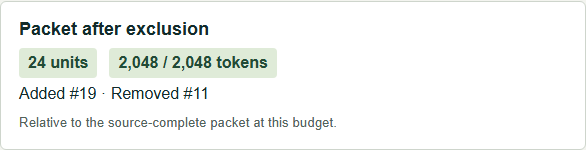
\includegraphics[width=\linewidth]{trace.png}\end{minipage}\hfill
\begin{minipage}[t]{.48\textwidth}\vspace{0pt}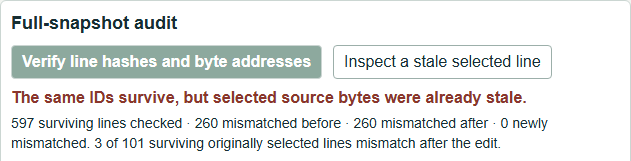
\includegraphics[width=\linewidth]{edit.png}\end{minipage}
\caption{Two running consoles. Left, excluding an execution source replaces unit 11 with unit 19 at the same cost. Right, a coding-agent edit retains the selected block IDs, yet the snapshot check detects incorrect line addresses in the original display. The audit operates separately from selection.}
\label{fig:ui}
\end{figure*}

\subsection{Three visitor scenarios}
\textit{Change the trace evidence.} Select q02 and inspect a unit's source ranges. Exclude an unused source to reuse its packet, then exclude the selected source. Unit 19 replaces unit 11. Comparing the maintained result with full recomputation checks the ordered IDs. A separate evaluation control then shows that all 60 annotated characters remain covered.

\textit{Change the budget or boundary.} Reduce the token budget and inspect which supporting range drops out. In q07 an exclusion touches only the indexed prefix boundary. The conservative plan recomputes, while the exact test establishes that the packet survives.

\textit{Follow a real code edit.} Switch to the edit console and choose a recorded case. In the first, a line shift preserves a 315-byte packet and its two block IDs. In the second, the edit intersects two of three blocks, leaving 74 of 507 bytes. In the third, all 14 IDs and 2,044 bytes survive. Auditing the underlying snapshots identifies three selected lines whose reported addresses were already wrong before the edit. Each outcome is a recorded example; the larger evaluation below estimates their prevalence on its stated cohort.

\section{Measurements and interpretation}
\subsection{Budgeted evidence recovery}
On 2,000 held-out ISETrace memory queries from 1,207 trajectories, all readers use the same candidate units and official source-span metric. Full Support is one when the union of selected source intervals contains every annotated gold interval. We average over five matched dense-retrieval seeds. The first-fit comparator uses the same graph-informed ranker and token costs. It receives the entire budget to admit later items that fit. This control isolates the effect of choosing the packet under a different objective.

\begin{table}[t]
\caption{Evidence recovery under a 2,048-token cap. Values are means across five matched seeds on the complete test.}
\centering\small
\begin{tabular}{lrr}\toprule
Selector & Support (\%) & Tokens/query\\\midrule
Full R-GCN, strict prefix & 78.60 & 1,854.95\\
No adjacency, strict prefix & 79.21 & 1,850.31\\
Full R-GCN, first-fit & 80.44 & 2,039.97\\
No adjacency, first-fit & 81.19 & 2,039.83\\\midrule
Dense order + exact packing & 75.25 & 2,038.61\\
Graph rank-weighted packing & 80.37 & 2,036.40\\
Graph utility/cost greedy & 82.31 & 2,034.63\\
Same-ranker first-fit & 82.19 & 2,039.30\\
Prefix + exact packing & 82.60 & 2,039.12\\
No adjacency + learned packing & 83.07 & 2,039.12\\
\bottomrule\end{tabular}
\label{tab:retrieval}
\end{table}

The full native relational graph model and its separately trained ablation without chunk adjacency are paired by seed, query, candidate set and cost. Our primary graph ordering with learned packing reaches 82.60\%, versus 82.19\% for its own first-fit (difference $+0.41$ points, crossed 95\% interval $[-0.23,1.08]$). Over six budgets from 256 to 8,192 tokens, normalized Full Support AUC is 70.992\% versus 70.565\% ($+0.427$ points, $[0.102,0.758]$).

The strongest tested hybrid uses the no-adjacency model's prefix and our learned utility. Against first-fit on that same native ranking, it gains 1.88 points ($[0.76,3.07]$) at 2,048 tokens. We selected this ordering after inspecting the budget curves. Sorting by absolute learned utility is a strong inexpensive alternative: its AUC is 71.204\%, against 71.324\% for exact packing ($+0.120$ points, $[-0.053,0.298]$). The trace console uses the primary 82.60\% configuration. All quoted retrieval measures concern evidence availability under a fixed cap.

We additionally rebuilt the visible graph halfway through execution. Among 901 questions in 657 trajectories whose complete support already existed, the primary graph ordering with first-fit recovered 84.73\%, versus 77.25\% for dense first-fit ($+7.48$ points, $[5.52,9.52]$), with a difference of 0.05 tokens per query. Exact packing reached 84.59\% ($-0.13$ points against graph first-fit, $[-1.07,0.80]$). For a stronger comparison, we rebuilt the native R-GCN input from the physically truncated histories and ran ten original checkpoints on the visible graphs. First-fit on the stronger native no-adjacency model attained 81.38\%, against 84.73\% for our first-fit ranking ($+3.35$ points, $[1.40,5.35]$), at 2,015 and 2,013 tokens, respectively. Filtering the terminal native ranking to visible units yielded 84.24\%: this shortcut overstated the causal baseline by 2.86 points ($[1.59,4.24]$). Query times are simulated because questions were written for completed histories. On all 1,845 questions in this evaluation panel, including those whose support had yet to appear, exact packing recovered 41.31\% halfway through execution.

\subsection{View maintenance on a live projection}
At 2,048 tokens the portable reader reproduced every ordered ID in all 40 frozen-model packets. Independent interval arithmetic matched the official evaluation in every case. Mean size was 2,043.15 tokens and 36 packets carried complete support. Exploratory budgets of 1,024 and 3,072 tokens gave 35 and 37 complete packets respectively.

We independently excluded each of the 2,528 query-source pairs from the initial snapshot. The indexed sufficient certificate served the old packet on 2,041 exclusions and recomputed the remaining 487. Ordered IDs matched fresh recomputation on every operation. Three conservative recalculations left the packet unchanged. The cache-hit rate was 80.74\% across exclusions and 77.80\% when each trace was weighted equally.

Both plans used identical SQLite data, native packing and precomputed features. Three interleaved repetitions gave 7,584 timed executions per plan. Aggregate full-recomputation time divided by certificate time was $5.16\times$, with a 95\% trajectory-bootstrap interval of $[4.36,6.17]$. Median latency fell from 280.25 to 9.30 microseconds and p95 from 540.29 to 352.82 microseconds. The dependency index added a mean 116 microseconds of setup per query. These are warm, single-host serving measurements. They exclude model training, feature extraction, browser rendering and evidence evaluation. The interactive portable implementation uses a Python optimizer to make the same decisions without native dependencies.

\balance
\begin{table}[t]
\caption{Exact reuse under independent hypothetical source exclusions. The final column counts additional reuse approvals beyond the fast boundary certificate.}
\centering\small
\begin{tabular}{rrrr}\toprule
Sources removed & Cases & Unchanged & Additional\\\midrule
1 & 2,528 & 2,044 & 3\\
2 & 97,676 & 68,336 & 232\\
3 & 4,000 & 1,991 & 12\\
8 & 4,000 & 890 & 17\\
\bottomrule\end{tabular}
\label{tab:exclusions}
\end{table}

The necessary-and-sufficient criterion (Table~\ref{tab:exclusions}) was also tested on 97,676 pairs of source deletions and 4,000 each of triples and eight-source sets. Together with the single exclusions this gave 108,204 comparisons. The criterion identified all 73,261 unchanged packets with zero false positives or negatives. It certified 264 additional unchanged packets compared with the conservative boundary test. Separately, exhaustive enumeration of 20,204 deletion sets on 320 small synthetic pools checked the predicted equivalence, including tied utilities. On the real panel an index monitoring only selected units happened to produce the correct outputs, although the counterexample above establishes its limits. The measured speedup belongs to the conservative single-source plan. Dynamic changes to rank, utility, cost or budget require a fresh snapshot or a separate maintenance argument.

\section{Serving memory during code edits}
We replayed 3,525 observed write attempts from Handoff Debt~\cite{handoff} on 37 issues across five Python repositories. Windows were selected around an observed read followed by a confirmed replacement. A separate integer view packs recent line blocks under a 2,048-byte cap. Whole-file invalidation permitted reuse in six of 2,820 attempts affecting a present path. Invalidation granularity and workload therefore matter to the benefit of caching.

A receipt locates the changed lines. We invalidate overlapping blocks and shift surviving addresses. A guard withholds displayed suffixes after clipping or coordinate discontinuities. Frozen on 24 issues, it retained 43,299 of 47,924 candidate lines on the other 13. Across 1,071 edits, range maintenance preserved 302 complete packets, versus 2 for file invalidation, 92 for symbol invalidation using Python syntax trees, and 287 for unique content matching against the new file. Issue-macro gains were 26.14 points over files ($[19.70,32.23]$), 17.92 over symbols ($[12.73,23.01]$) and 1.56 over content ($[-2.19,5.39]$). Content matching retained more individual bytes. All 25,912 surviving lines checked on edited paths matched their subsequent snapshots. A coding-task success gain remains unestablished.

On 40 ISETrace projections we also replayed arrivals at the original message positions. Caching the optimal suffix for each capacity and updating it after new units gave exactly the full solution at all 2,336 steps and reduced selector time by $3.88\times$ ($[3.16,4.83]$) on one CPU. This separate operator study fixes costs, ranks and utilities throughout each replay; it excludes encoder and graph-scoring time. Together, the two visitor scenarios expose packet identity, source validity and the cost of maintaining each.

\section*{Acknowledgments}
OpenAI Codex assisted with the design and implementation of the methods in Sections II and III, experimental pipelines and analyses in Sections IV and V, preparation of the figures and demonstration, and drafting of the manuscript. Reported measurements were computed by the cited evaluation code and checked against persisted per-query or per-edit results.

\bibliographystyle{IEEEtran}
\bibliography{sources}
\end{document}
